%
% buchcover.tex -- Cover für das Buch Felder
%
% (c) 2018-2025 Prof Dr Andreas Müller, Hochschule Rapperswil
%
\documentclass[11pt]{standalone}
\usepackage{tikz}
\usepackage{times}
\usepackage{geometry}
\usepackage[utf8]{inputenc}
\usepackage[T1]{fontenc}
\usepackage{times}
\usepackage{amsmath,amscd}
\usepackage{amssymb}
\usepackage{amsfonts}
\usepackage{german}
\usepackage{txfonts}
\usepackage{ifthen}
\usepackage{qrcode}
\usetikzlibrary{math,fadings}
\geometry{papersize={417mm,278mm},total={417mm,278mm},top=72.27pt, bottom=0pt, left=72.27pt, right=0pt}
\newboolean{guidelines}
\setboolean{guidelines}{true}
\setboolean{guidelines}{false}
\newboolean{teilnehmer}
\setboolean{teilnehmer}{false}
\setboolean{teilnehmer}{true}

\begin{document}
\begin{tikzpicture}[>=latex, scale=1]
\tikzmath{
	real \ruecken, \einschlag, \gelenk, \breite, \hoehe;
	\ruecken = 4.5;
	\einschlag = 1.6;
	\gelenk = 0.8;
	\breite = 16.7;
	\hoehe = 24.6;
	real \bogengreite, \bogenhoehe;
	\bogenbreite = 2 * (\breite + \einschlag + \gelenk) + \ruecken;
	\bogenhoehe = 2 * \einschlag + \hoehe;
}


\draw[fill=blue] (0,0) rectangle ({\bogenbreite},{\bogenhoehe});
\hsize=13.6cm

\begin{scope}
\clip (0,0) rectangle({\bogenbreite},{0.48*\bogenhoehe});

\coordinate (A) at (0,0);
\coordinate (B) at ({0.9*\bogenbreite},0);
\coordinate (C) at (\bogenbreite,0);
\coordinate (D) at (\bogenbreite,{0.2*\bogenhoehe});
\coordinate (E) at (\bogenbreite,{0.55*\bogenhoehe});
\coordinate (F) at ({0.2*\bogenbreite},{0.55*\bogenhoehe});
\coordinate (G) at (0,{0.55*\bogenhoehe});
\coordinate (H) at (0,{0.2*\bogenhoehe});


\begin{scope}
\node at ({0.75*\bogenbreite},8.0)
	{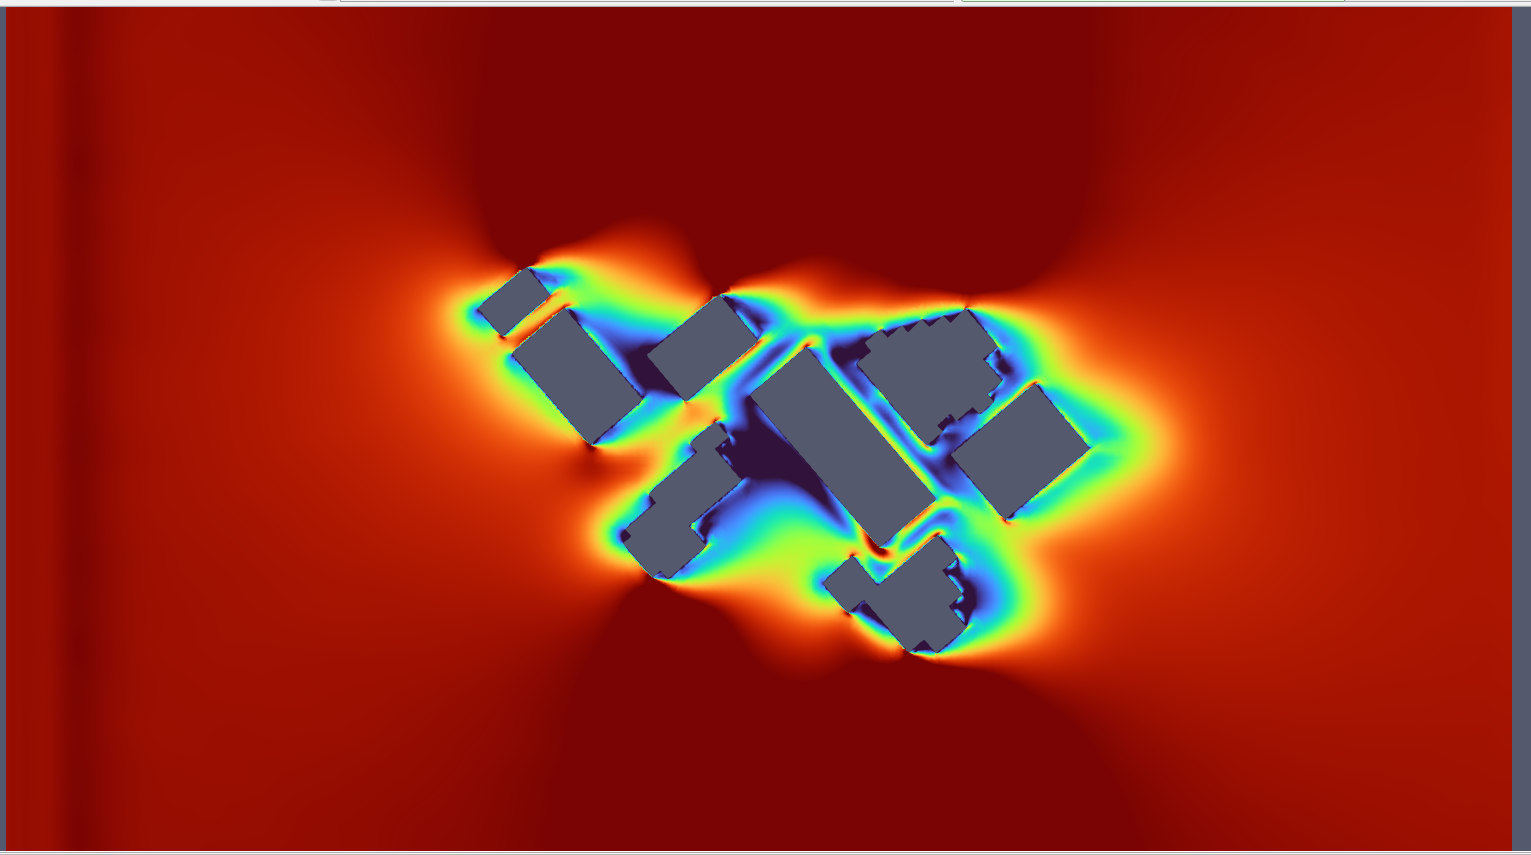
\includegraphics[width=38cm]{frontimage-flipped.png}};
\end{scope}

\begin{scope}
\clip (0,0) -- ({0.5*\bogenbreite},0) -- ++(0,{0.54*\bogenhoehe})
	-- (0,{0.5*\bogenhoehe}) -- cycle;
\node at ({0.22*\bogenbreite},8.3)
	{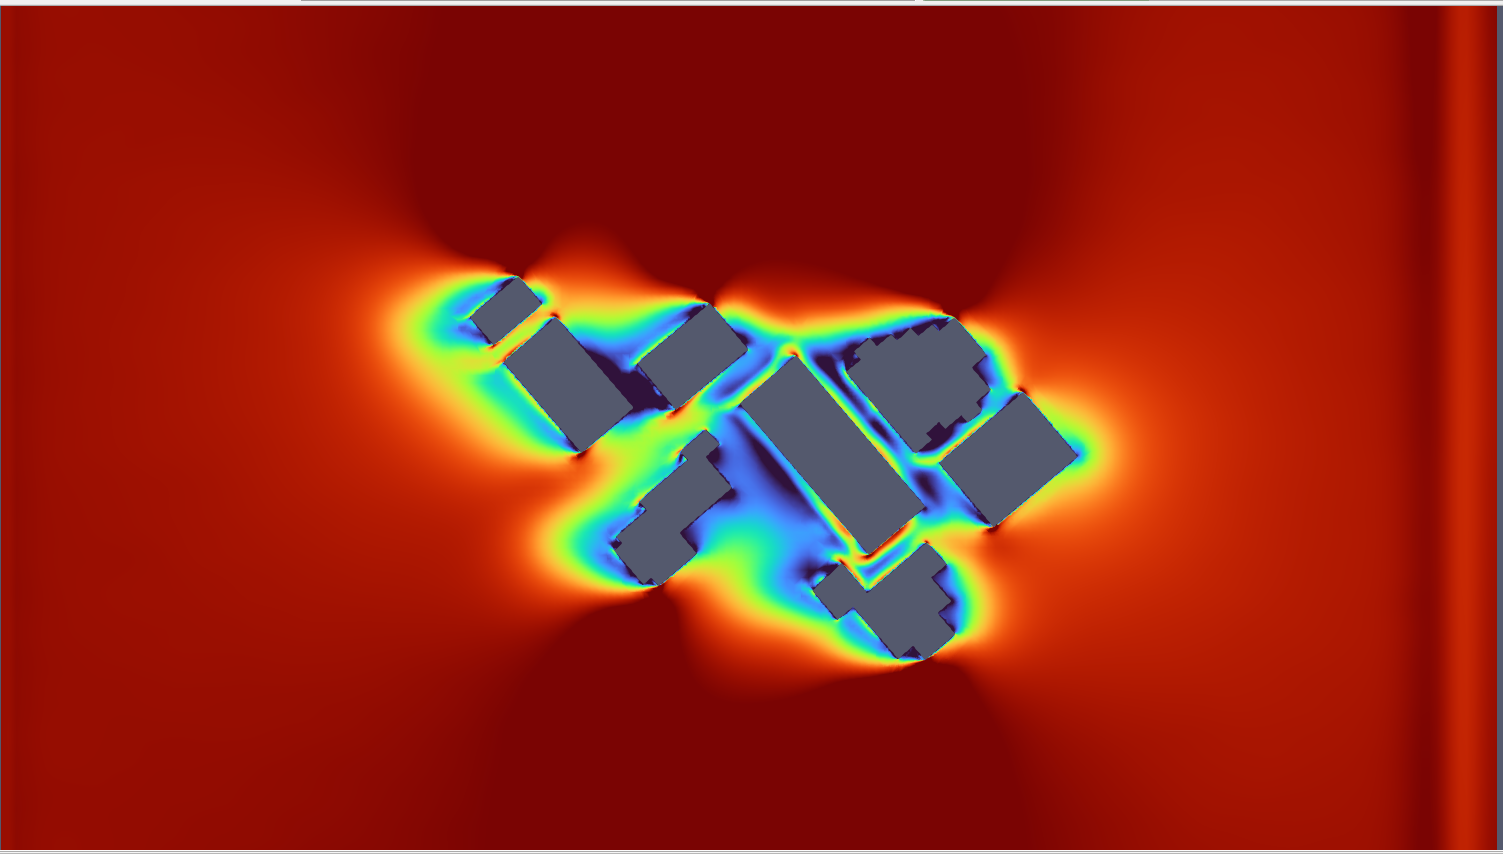
\includegraphics[width=38cm]{backimage-flipped.png}};
\end{scope}

%
% 3.336cm = (2*(\einschlag+\breite+\gelenk)+\ruecken)*0.08
%
\node at ({0.5*\bogenbreite},{0.24*\bogenhoehe})
	{
\includegraphics[width=3.336cm]{ruecken1.png}};

\end{scope}

\node at ({\einschlag+2*\gelenk+\ruecken+1.5*\breite},24.3)
	[color=white,scale=1]
	{\hbox to\hsize{\hfill%
	\sf \fontsize{24}{24}\selectfont Mathematisches Seminar}};

\node at ({\einschlag+2*\gelenk+\ruecken+1.5*\breite},21.9)
	[color=white,scale=1]
	{\hbox to\hsize{\hfill%
	\sf \fontsize{51}{51}\selectfont Felder}};

\node at ({\einschlag+2*\gelenk+\ruecken+1.5*\breite},19.7)
	[color=white,scale=1]
	{\hbox to\hsize{\hfill%
	\sf \fontsize{13}{5}\selectfont Andreas Müller}};

\def\teilnehmer#1#2{
\node at ({\einschlag+2*\gelenk+\ruecken+1.5*\breite},{18.4-(#1)*0.65})
	[color=white,scale=1]
	{\hbox to\hsize{\hfill%
	\sf \fontsize{13}{5}\selectfont
	{#2}%
	}};
}

\ifthenelse{\boolean{teilnehmer}}{
%
% teilnehmer.tex -- Liste der Seminarteilnehmer auf der Titelseite
%
% (c) 2025 Prof Dr Andreas Müller, OST Ostschweizer Fachhochschule
%
Sofia Aaltonen,		% B
Emir Arslan, 		% B
Jero Barahona%,		% E
\\
Ricardo Barbosa,	% B
Damian Birchler,	% EEU
Flurin Brechbühler%,	% E
\\
Nino Briker,		% E
Philip Brun,		% E
Domenico Cardini%,	% EEU
\\
Roman Cvijanovic,	% I
Nicola Dall'Acqua,	% I
Yanick Diggelmann%,	% E
\\
Robin Eberle,		% MSE
Sebastian Eggli,	% EEU
Damien Flury,		% I
Laurin Heitzer%,		% E
\\
Andrin Kälin,		% E
Shaarujan Kamalanathan,	% E
Alain Keller%,		% MSE
\\
Martina Knobel,		% E
Gian Kraus,		% E
Patrik Müller,		% MSE
Joël Rechsteiner%,	% MSE (extern)
\\
Mike Peng,		% E
Andrin Rütsche,		% E
Sagithiya Saseekaran%,	% B
\\
Michael Schmid,		% MSE
Lukas Schöpf,		% MSE
Fabian Steiner,		% E
Loris Trüb%,		% EEU
\\
Raphael Unterer,	% MSE
Pascal Widmer,		% E
Tobias Zuber%,		% M-I
\\

}{}
 
%\node at (0,3) [color=white] {\sf \LARGE Mathematisches Seminar 2017};

% Rücken
\node at ({\bogenbreite/2 + 0.00},18.5) [color=white,rotate=-90]
	{\sf\fontsize{35}{0}\selectfont Felder\strut};

% Buchrückseite
\node at ({\einschlag+0.5*\breite},18.6) [color=white] {\sf
\fontsize{13}{16}\selectfont
\vbox{%
\parindent=0pt
%\raggedright
Das Mathematische Seminar der Ostschweizer Fachhochschule
in Rapperswil hat sich im Frühjahrssemester 2025 dem Thema
Felder
zugewandt.
Ziel war, die mathematischen Grundkonzepte und Gemeinsamkeiten 
von Vektor- und Skalarfeldern in Physik und Technik zu ergründen.
Dieses Buch bringt das Skript des Vorlesungsteils mit den von den
Seminarteilnehmern beigetragenen Seminararbeiten zusammen.

\medskip

Zum Umschlagbild: Die Windströmung um die Gebäude der OST kann mit
einem Softwarepaket wie OpenFOAM berechnet werden, wie es in Kapitel~24
vorgestellt wird.
Der Buchdeckel zeigt die %Ost-Westkomponente der
Strömungsgeschwindigkeit
des Windes auf 5\,m Höhe über Grund bei Westwind, auf der Rückseite (unten)
wurde mit einer Ostströmung gerechnet.

%Zum Umschlagbild: Eine Wendeltreppe entsteht aus horizontalen Treppenstufen,
%die spiralförmig um die vertikale Achse angeordnet sind.
%Sie bilden eine Wendelfläche oder Helikoide.
%In Kapitel~17 wird gezeigt, dass sie auch eine Minimalfläche ist, 
%also die Form, die eine Seifenhaut annimmt, die sich zwischen einem
%spiralförmig gebogenen Draht und einer Achse aufspannt.
}};

\def\qrbreite{3}
\def\qrrightoffset{0}
\def\qrbottomoffset{1.5}

\fill[color=white]
        ({\einschlag+(\breite+13.6)/2-\qrbreite-0.1},{\einschlag+\qrbottomoffset-0.1})
        rectangle
        ({\einschlag+(\breite+13.6)/2+0.1},{\einschlag+\qrbottomoffset+\qrbreite+0.1});

\node at ({\einschlag+(\breite+13.6)/2-\qrbreite/2},{\einschlag+\qrbottomoffset+\qrbreite/2}) {
\qrcode[height=3cm]{https://mathsem.ch/jahre/2025/SeminarFelder.pdf}
};
\node at ({\einschlag+(\breite+13.6)/2-\qrbreite/2},{\einschlag+\qrbottomoffset+\qrbreite/2}) {

\includegraphics[width=10mm]{mathman.png}
};

\ifthenelse{\boolean{guidelines}}{
\draw[white] (0,{\einschlag})--({\bogenbreite},{\einschlag});
\draw[white] (0,{\bogenhoehe-\einschlag})--({\bogenbreite},{\bogenhoehe-\einschlag});

\draw[white] ({\einschlag},0)--({\einschlag},{\bogenhoehe});
\draw[white] ({\einschlag+\breite},0)--({\einschlag+\breite},{\bogenhoehe});
\draw[white] ({\einschlag+\breite+\gelenk},0)--({\einschlag+\breite+\gelenk},{\bogenhoehe});
\draw[white] ({\bogenbreite-\einschlag-\breite-\gelenk},0)--({\bogenbreite-\einschlag-\breite-\gelenk},{\bogenhoehe});
\draw[white] ({\bogenbreite-\einschlag-\breite},0)--({\bogenbreite-\einschlag-\breite},{\bogenhoehe});
\draw[white] ({\bogenbreite-\einschlag},0)--({\bogenbreite-\einschlag},{\bogenhoehe});
}{}

\end{tikzpicture}
\end{document}
